\section{Paper 5}

\title[PhD Defence]{
    {\Huge Paper 5} \\
    \vspace{2mm}
    {\Large Stochastic Analysis of Control Systems}\\
    {\Large Subject to Communication and Computation Faults}
}
\author[Nils Vreman]{
    Nils Vreman \\
    \vspace{3mm}
    {\large Martina Maggio}
}
\date[EMSOFT 2023]{
    Submitted to the International Conference on Embedded Software (EMSOFT), 2023\\
}
\notitlelogo
\frame[plain,noframenumbering]{\titlepage}


% a frame with figures using \only to show them one by one
\begin{frame}
    \frametitle{Fault Models}
    \begin{figure}
        \centering
        \only<1>{\def \delta {0.15}
\def \circlesizecm {0.5cm}
\def \circleshiftcm {0.125cm}
\def \armlength {0.625}
\def \armwidthcm {0.1cm}
\def \bodywidthcm {0.5cm}

\begin{tikzpicture}
\tikzstyle{task} = [draw,thick,fill=white,align=center]
\tikzstyle{turbine} = [circle,ultra thick,draw,fill=white,minimum size=\circlesizecm,inner sep=0pt,outer sep=0pt]

%%% TASKS %%%

\node[task,opacity=0.3] (t1) at (-1.5+0*\delta,1.6-0*\delta) {\textcolor{white}{Task $\#3$} \\\textcolor{white}{\faFileCode[regular]}};
\node[task,opacity=0.6] (t2) at (-1.5+1*\delta,1.6-1*\delta) {\textcolor{white}{Task $\#2$} \\\textcolor{white}{\faFileCode[regular]}};
\node[task,opacity=1.0] (t3) at (-1.5+2*\delta,1.6-2*\delta) {Task $\#1$ \\\faFileCode[regular]};

\node[task,opacity=0.3] (ct1) at (1.5+0*\delta,1.6-0*\delta) {\textcolor{white}{Control Task $\#3$} \\\textcolor{white}{\faFileCode[regular]}};
\node[task,opacity=0.6] (ct2) at (1.5+1*\delta,1.6-1*\delta) {\textcolor{white}{Control Task $\#2$} \\\textcolor{white}{\faFileCode[regular]}};
\node[task,opacity=1.0] (ct3) at (1.5+2*\delta,1.6-2*\delta) {\textcolor{blue}{Control Task $\#1$} \\\textcolor{blue}{\faFileCode[regular]}};

%%% CYBER %%%

\node[thick, align=center] (rtos) at (-0.1,0.25) {Real-Time Operating System};
\node[thick, draw, align=center, rotate=90, text width=2.75cm] (hwi) at (4.1,0.87) {HW Interfaces};
\node[thick, fit=(rtos)(t1)(ct1)(ct3),draw,yshift=1.5mm,xshift=0.75mm] (sw) {};
\node[thick, draw, above left] (clock) at (sw.south east) {\faClock[regular]};
\node[thick, fit=(sw)(hwi), inner sep=7pt, draw] (hw) {};
\node[thick, above left, xshift=2.40cm, yshift=0.5mm] (hw-label) at (hw.south west) {Hardware};
\node[thick, draw, above right] (hwclock) at (hw.south west)  {\faClock[regular]};

%%% PHYSICAL %%%

\node[task, minimum width=2.125cm, minimum height=2.125cm] (phys) at (7.0,0.875) {};
% body
\node[
    draw,
    rounded corners=3pt,
    fill=black,
    minimum width=\bodywidthcm,
    minimum height=\bodywidthcm,
    name path=B] (body) at (phys) {};

% upper left turbine
\node[turbine, anchor=south east] (dronenw) at ([xshift=-\circleshiftcm, yshift=\circleshiftcm]body.north west) {};
\draw[name path=NW] ([yshift=-\armwidthcm]body.north west)..controls($(phys) + (-\armlength, \armlength)$)..([xshift=\armwidthcm]body.north west);
\tikzfillbetween [of=NW and B] {};
\draw[fill=black, rotate=75] (dronenw) ellipse (0.175cm and 0.025cm);
\draw[fill=black, rotate=165] (dronenw) ellipse (0.175cm and 0.025cm);
        
% upper right turbine
\node[turbine, anchor=south west] (dronene) at ([xshift=\circleshiftcm, yshift=\circleshiftcm]body.north east) {};
\draw[name path=NE] ([xshift=-\armwidthcm]body.north east)..controls($(phys) + (\armlength, \armlength)$)..([yshift=-\armwidthcm]body.north east);
\tikzfillbetween [of=NE and B] {};
\draw[fill=black, rotate=75] (dronene) ellipse (0.175cm and 0.025cm);
\draw[fill=black, rotate=165] (dronene) ellipse (0.175cm and 0.025cm);

% lower right turbine
\node[turbine, anchor=north west] (dronese) at ([xshift=\circleshiftcm, yshift=-\circleshiftcm]body.south east) {};
\draw[name path=SE] ([yshift=\armwidthcm]body.south east)..controls($(phys) + (\armlength, -\armlength)$)..([xshift=-\armwidthcm]body.south east);
\tikzfillbetween [of=SE and B] {};
\draw[fill=black, rotate=75] (dronese) ellipse (0.175cm and 0.025cm);
\draw[fill=black, rotate=165] (dronese) ellipse (0.175cm and 0.025cm);

% lower left turbine
\node[turbine, anchor=north east] (dronesw) at ([xshift=-\circleshiftcm, yshift=-\circleshiftcm]body.south west) {};
\draw[name path=SW] ([xshift=\armwidthcm]body.south west)..controls($(phys) + (-\armlength, -\armlength)$)..([yshift=\armwidthcm]body.south west);
\tikzfillbetween [of=SW and B] {};
\draw[fill=black, rotate=75] (dronesw) ellipse (0.175cm and 0.025cm);
\draw[fill=black, rotate=165] (dronesw) ellipse (0.175cm and 0.025cm);

% Clock
\node[task, above left] (time) at (phys.south east) {\faClock[regular]};

%%% ARROWS %%%

\draw[thick, -latex] ([yshift=0.65cm]hwi.south) to node[yshift=0.85cm,xshift=1mm,rotate=90] {\textcolor{blue}{Actuation}} ([yshift=0.65cm]phys.west);
\draw[thick, -latex] ([yshift=-0.65cm]phys.west) to node[yshift=-0.75cm,xshift=1mm,rotate=90] {\textcolor{blue}{Sensing}} ([yshift=-0.65cm]hwi.south);

\end{tikzpicture}
}%
        \only<2>{\def \delta {0.15}
\def \circlesizecm {0.5cm}
\def \circleshiftcm {0.125cm}
\def \armlength {0.625}
\def \armwidthcm {0.1cm}
\def \bodywidthcm {0.5cm}

\begin{tikzpicture}
\tikzstyle{task} = [draw,thick,fill=white,align=center]
\tikzstyle{turbine} = [circle,ultra thick,draw,fill=white,minimum size=\circlesizecm,inner sep=0pt,outer sep=0pt]

%%% TASKS %%%

\node[task,opacity=0.3] (t1) at (-1.5+0*\delta,1.6-0*\delta) {\textcolor{white}{Task $\#3$} \\\textcolor{white}{\faFileCode[regular]}};
\node[task,opacity=0.6] (t2) at (-1.5+1*\delta,1.6-1*\delta) {\textcolor{white}{Task $\#2$} \\\textcolor{white}{\faFileCode[regular]}};
\node[task,opacity=1.0] (t3) at (-1.5+2*\delta,1.6-2*\delta) {Task $\#1$ \\\faFileCode[regular]};

\node[task,opacity=0.3] (ct1) at (1.5+0*\delta,1.6-0*\delta) {\textcolor{white}{Control Task $\#3$} \\\textcolor{white}{\faFileCode[regular]}};
\node[task,opacity=0.6] (ct2) at (1.5+1*\delta,1.6-1*\delta) {\textcolor{white}{Control Task $\#2$} \\\textcolor{white}{\faFileCode[regular]}};
\node[task,opacity=1.0] (ct3) at (1.5+2*\delta,1.6-2*\delta) {Control Task $\#1$ \\\faFileCode[regular]};

%%% CYBER %%%

\node[thick, align=center] (rtos) at (-0.1,0.25) {Real-Time Operating System};
\node[thick, draw, align=center, rotate=90, text width=2.75cm] (hwi) at (4.1,0.87) {HW Interfaces};
\node[thick, fit=(rtos)(t1)(ct1)(ct3),draw,yshift=1.5mm,xshift=0.75mm] (sw) {};
\node[thick, draw, above left] (clock) at (sw.south east) {\faClock[regular]};
\node[thick, fit=(sw)(hwi), inner sep=7pt, draw] (hw) {};
\node[thick, above left, xshift=2.40cm, yshift=0.5mm] (hw-label) at (hw.south west) {Hardware};
\node[thick, draw, above right] (hwclock) at (hw.south west)  {\faClock[regular]};

%%% PHYSICAL %%%

\node[task, minimum width=2.125cm, minimum height=2.125cm, draw=hicolour] (phys) at (7.0,0.875) {};

% body
\node[
    draw,
    rounded corners=3pt,
    fill=black,
    minimum width=\bodywidthcm,
    minimum height=\bodywidthcm,
    name path=B] (body) at (phys) {};

% upper left turbine
\node[turbine, anchor=south east] (dronenw) at ([xshift=-\circleshiftcm, yshift=\circleshiftcm]body.north west) {};
\draw[name path=NW] ([yshift=-\armwidthcm]body.north west)..controls($(phys) + (-\armlength, \armlength)$)..([xshift=\armwidthcm]body.north west);
\tikzfillbetween [of=NW and B] {};
\draw[fill=black, rotate=75] (dronenw) ellipse (0.175cm and 0.025cm);
\draw[fill=black, rotate=165] (dronenw) ellipse (0.175cm and 0.025cm);
        
% upper right turbine
\node[turbine, anchor=south west] (dronene) at ([xshift=\circleshiftcm, yshift=\circleshiftcm]body.north east) {};
\draw[name path=NE] ([xshift=-\armwidthcm]body.north east)..controls($(phys) + (\armlength, \armlength)$)..([yshift=-\armwidthcm]body.north east);
\tikzfillbetween [of=NE and B] {};
\draw[fill=black, rotate=75] (dronene) ellipse (0.175cm and 0.025cm);
\draw[fill=black, rotate=165] (dronene) ellipse (0.175cm and 0.025cm);

% lower right turbine
\node[turbine, anchor=north west] (dronese) at ([xshift=\circleshiftcm, yshift=-\circleshiftcm]body.south east) {};
\draw[name path=SE] ([yshift=\armwidthcm]body.south east)..controls($(phys) + (\armlength, -\armlength)$)..([xshift=-\armwidthcm]body.south east);
\tikzfillbetween [of=SE and B] {};
\draw[fill=black, rotate=75] (dronese) ellipse (0.175cm and 0.025cm);
\draw[fill=black, rotate=165] (dronese) ellipse (0.175cm and 0.025cm);

% lower left turbine
\node[turbine, anchor=north east] (dronesw) at ([xshift=-\circleshiftcm, yshift=-\circleshiftcm]body.south west) {};
\draw[name path=SW] ([xshift=\armwidthcm]body.south west)..controls($(phys) + (-\armlength, -\armlength)$)..([yshift=\armwidthcm]body.south west);
\tikzfillbetween [of=SW and B] {};
\draw[fill=black, rotate=75] (dronesw) ellipse (0.175cm and 0.025cm);
\draw[fill=black, rotate=165] (dronesw) ellipse (0.175cm and 0.025cm);

% Clock
{\color{hicolour}\node[task, above left] (time) at (phys.south east) {\faClock[regular]};}

{\color{hicolour}\node[] (phystmp) at ([yshift=-0.25cm]phys.south) {Plant};}

%%% ARROWS %%%

\draw[thick, -latex] ([yshift=0.65cm]hwi.south) to node[yshift=0.85cm,xshift=1mm,rotate=90] {Actuation} ([yshift=0.65cm]phys.west);
\draw[thick, -latex] ([yshift=-0.65cm]phys.west) to node[yshift=-0.75cm,xshift=1mm,rotate=90] {Sensing} ([yshift=-0.65cm]hwi.south);

\end{tikzpicture}
}%
        \only<3>{\def \delta {0.15}

\begin{tikzpicture}
\tikzstyle{task} = [draw, fill=white,align=center]

%%%%%%%%%%%
%%% CPS %%%
%%%%%%%%%%%

%%% TASKS %%%

\node[task,] (t1) at (-2+0*\delta,1.6-0*\delta) {Task $\#1$ \\\faFileCode[regular]};
\node[task,] (t2) at (-2+1*\delta,1.6-1*\delta) {Task $\#2$ \\\faFileCode[regular]};
\node[task,] (t3) at (-2+2*\delta,1.6-2*\delta) {Task $\#3$ \\\faFileCode[regular]};

\node[task,] (ct1) at (1+0*\delta,1.6-0*\delta) {Control-Task $\#1$ \\\faFileCode[regular]};
\node[task,] (ct2) at (1+1*\delta,1.6-1*\delta) {Control-Task $\#2$ \\\faFileCode[regular]};
\node[task,] (ct3) at (1+2*\delta,1.6-2*\delta) {Control-Task $\#3$ \\\faFileCode[regular]};

%%% CYBER %%%

\node[align=center] (rtos) at (-0.2,0.15)  {Real-Time Operating System};
\node[draw, align=center, rotate=90, text width=3.0cm] (hw)   at (3.35,0.775) {HW interfaces};
\node[fit=(rtos)(t1)(ct1)(ct3),draw,yshift=1.5mm] (sw) {};
\node[draw, above left] (clock) at (sw.south east)  {\faClock[regular]};
{\color{lqgcolour}\node[thick, fit=(sw)(hw),draw] (board) {};}
{\color{lqgcolour}\node[above left, xshift=1.8cm] (borad-label) at (board.south west) {Board};}
{\color{lqgcolour}\node[draw, above right] (clockboard) at (board.south west)  {\faClock[regular]};}

%%% PHYSICAL %%%

\node[thick, draw ,align=center] (phys) at (6,0.775) {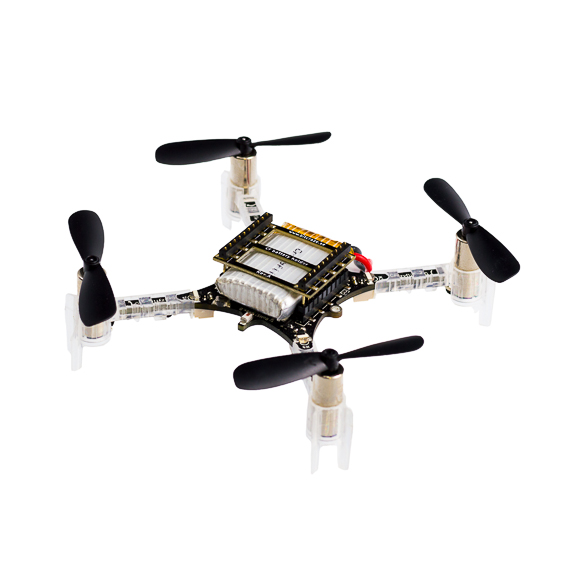
\includegraphics[scale=0.4]{figs/topic/crazyflie.jpg}};
\node[draw, above left] (time) at (phys.south east)  {\faClock[regular]};

%%% ARROWS %%%

\draw[-latex] ([yshift=0.65cm]hw.south) to node[yshift=0.85cm,rotate=90]{actuation} ([yshift=0.65cm]phys.west);
\draw[-latex] ([yshift=-0.65cm]phys.west) to node[yshift=-0.85cm, rotate=90]{sensing} ([yshift=-0.65cm]hw.south);

\end{tikzpicture}
}%
        \only<4>{\def \delta {0.15}
\def \circlesizecm {0.5cm}
\def \circleshiftcm {0.125cm}
\def \armlength {0.625}
\def \armwidthcm {0.1cm}
\def \bodywidthcm {0.5cm}

\begin{tikzpicture}
\tikzstyle{task} = [draw,thick,fill=white,align=center]
\tikzstyle{turbine} = [circle,ultra thick,draw,fill=white,minimum size=\circlesizecm,inner sep=0pt,outer sep=0pt]

%%% TASKS %%%

\node[task,opacity=0.3] (t1) at (-1.5+0*\delta,1.6-0*\delta) {\textcolor{white}{Task $\#3$} \\\textcolor{white}{\faFileCode[regular]}};
\node[task,opacity=0.6] (t2) at (-1.5+1*\delta,1.6-1*\delta) {\textcolor{white}{Task $\#2$} \\\textcolor{white}{\faFileCode[regular]}};
\node[task,opacity=1.0] (t3) at (-1.5+2*\delta,1.6-2*\delta) {Task $\#1$ \\\faFileCode[regular]};

\node[task,opacity=0.3] (ct1) at (1.5+0*\delta,1.6-0*\delta) {\textcolor{white}{Control Task $\#3$} \\\textcolor{white}{\faFileCode[regular]}};
\node[task,opacity=0.6] (ct2) at (1.5+1*\delta,1.6-1*\delta) {\textcolor{white}{Control Task $\#2$} \\\textcolor{white}{\faFileCode[regular]}};
\node[task,opacity=1.0] (ct3) at (1.5+2*\delta,1.6-2*\delta) {\textcolor{hicolour}{Control Task $\#1$} \\\textcolor{hicolour}{\faFileCode[regular]}};

%%% CYBER %%%

\node[thick, align=center] (rtos) at (-0.1,0.25) {Real-Time Operating System};
\node[thick, draw, align=center, rotate=90, text width=2.75cm] (hwi) at (4.1,0.87) {HW Interfaces};
\node[thick, fit=(rtos)(t1)(ct1)(ct3),draw,yshift=1.5mm,xshift=0.75mm] (sw) {};
\node[thick, draw, above left] (clock) at (sw.south east) {\faClock[regular]};
\node[thick, fit=(sw)(hwi), inner sep=7pt, draw] (hw) {};
\node[thick, above left, xshift=2.40cm, yshift=0.5mm] (hw-label) at (hw.south west) {Hardware};
\node[thick, draw, above right] (hwclock) at (hw.south west)  {\faClock[regular]};

%%% PHYSICAL %%%

\node[task, minimum width=2.125cm, minimum height=2.125cm] (phys) at (7.0,0.875) {};
% body
\node[
    draw,
    rounded corners=3pt,
    fill=black,
    minimum width=\bodywidthcm,
    minimum height=\bodywidthcm,
    name path=B] (body) at (phys) {};

% upper left turbine
\node[turbine, anchor=south east] (dronenw) at ([xshift=-\circleshiftcm, yshift=\circleshiftcm]body.north west) {};
\draw[name path=NW] ([yshift=-\armwidthcm]body.north west)..controls($(phys) + (-\armlength, \armlength)$)..([xshift=\armwidthcm]body.north west);
\tikzfillbetween [of=NW and B] {};
\draw[fill=black, rotate=75] (dronenw) ellipse (0.175cm and 0.025cm);
\draw[fill=black, rotate=165] (dronenw) ellipse (0.175cm and 0.025cm);
        
% upper right turbine
\node[turbine, anchor=south west] (dronene) at ([xshift=\circleshiftcm, yshift=\circleshiftcm]body.north east) {};
\draw[name path=NE] ([xshift=-\armwidthcm]body.north east)..controls($(phys) + (\armlength, \armlength)$)..([yshift=-\armwidthcm]body.north east);
\tikzfillbetween [of=NE and B] {};
\draw[fill=black, rotate=75] (dronene) ellipse (0.175cm and 0.025cm);
\draw[fill=black, rotate=165] (dronene) ellipse (0.175cm and 0.025cm);

% lower right turbine
\node[turbine, anchor=north west] (dronese) at ([xshift=\circleshiftcm, yshift=-\circleshiftcm]body.south east) {};
\draw[name path=SE] ([yshift=\armwidthcm]body.south east)..controls($(phys) + (\armlength, -\armlength)$)..([xshift=-\armwidthcm]body.south east);
\tikzfillbetween [of=SE and B] {};
\draw[fill=black, rotate=75] (dronese) ellipse (0.175cm and 0.025cm);
\draw[fill=black, rotate=165] (dronese) ellipse (0.175cm and 0.025cm);

% lower left turbine
\node[turbine, anchor=north east] (dronesw) at ([xshift=-\circleshiftcm, yshift=-\circleshiftcm]body.south west) {};
\draw[name path=SW] ([xshift=\armwidthcm]body.south west)..controls($(phys) + (-\armlength, -\armlength)$)..([yshift=\armwidthcm]body.south west);
\tikzfillbetween [of=SW and B] {};
\draw[fill=black, rotate=75] (dronesw) ellipse (0.175cm and 0.025cm);
\draw[fill=black, rotate=165] (dronesw) ellipse (0.175cm and 0.025cm);

% Clock
\node[task, above left] (time) at (phys.south east) {\faClock[regular]};

%%% ARROWS %%%

{\color{hicolour}\draw[thick, -latex] ([yshift=0.65cm]hwi.south) to node[yshift=0.85cm,xshift=1mm,rotate=90] {\phantom{Actuation}} ([yshift=0.65cm]phys.west);}
{\color{red}\draw[thick, -latex] ([yshift=-0.65cm]phys.west) to node[yshift=-0.75cm,xshift=1mm,rotate=90] {\phantom{Sensing}} ([yshift=-0.65cm]hwi.south);}

%%% Packets
\node (packetS) at ([xshift=-0.25cm, yshift=-0.4cm]phys.west) {\textcolor{red}{\faBox}};

\node (packetA) at ([xshift=0.5cm, yshift=0.9cm]hwi.south) {\textcolor{hicolour!85!white}{\faBox}};


\end{tikzpicture}
}%
        \only<5>{\def \delta {0.15}
\def \circlesizecm {0.5cm}
\def \circleshiftcm {0.125cm}
\def \armlength {0.625}
\def \armwidthcm {0.1cm}
\def \bodywidthcm {0.5cm}

\begin{tikzpicture}
\tikzstyle{task} = [draw,thick,fill=white,align=center]
\tikzstyle{turbine} = [circle,ultra thick,draw,fill=white,minimum size=\circlesizecm,inner sep=0pt,outer sep=0pt]

%%% TASKS %%%

\node[task,opacity=0.3] (t1) at (-1.5+0*\delta,1.6-0*\delta) {\textcolor{white}{Task $\#3$} \\\textcolor{white}{\faFileCode[regular]}};
\node[task,opacity=0.6] (t2) at (-1.5+1*\delta,1.6-1*\delta) {\textcolor{white}{Task $\#2$} \\\textcolor{white}{\faFileCode[regular]}};
\node[task,opacity=1.0] (t3) at (-1.5+2*\delta,1.6-2*\delta) {Task $\#1$ \\\faFileCode[regular]};

\node[task,opacity=0.3] (ct1) at (1.5+0*\delta,1.6-0*\delta) {\textcolor{white}{Control Task $\#3$} \\\textcolor{white}{\faFileCode[regular]}};
\node[task,opacity=0.6] (ct2) at (1.5+1*\delta,1.6-1*\delta) {\textcolor{white}{Control Task $\#2$} \\\textcolor{white}{\faFileCode[regular]}};
\node[task,opacity=1.0] (ct3) at (1.5+2*\delta,1.6-2*\delta) {Control Task $\#1$ \\\faFileCode[regular]};

%%% CYBER %%%

{\color{lqgcolour}\node[thick, align=center] (rtos) at (-0.1,0.25) {Real-Time Operating System};}
\node[thick, draw, align=center, rotate=90, text width=2.75cm] (hwi) at (4.1,0.87) {HW Interfaces};
{\color{lqgcolour}\node[thick, fit=(rtos)(t1)(ct1)(ct3),draw,yshift=1.5mm,xshift=0.75mm] (sw) {};}
{\color{lqgcolour}\node[thick, draw, above left] (clock) at (sw.south east) {\faClock[regular]};}
\node[thick, fit=(sw)(hwi), inner sep=7pt, draw] (hw) {};
\node[thick, above left, xshift=2.40cm, yshift=0.5mm] (hw-label) at (hw.south west) {Hardware};
\node[thick, draw, above right] (hwclock) at (hw.south west)  {\faClock[regular]};

%%% PHYSICAL %%%

\node[task, minimum width=2.125cm, minimum height=2.125cm] (phys) at (7.0,0.875) {};
% body
\node[
    draw,
    rounded corners=3pt,
    fill=black,
    minimum width=\bodywidthcm,
    minimum height=\bodywidthcm,
    name path=B] (body) at (phys) {};

% upper left turbine
\node[turbine, anchor=south east] (dronenw) at ([xshift=-\circleshiftcm, yshift=\circleshiftcm]body.north west) {};
\draw[name path=NW] ([yshift=-\armwidthcm]body.north west)..controls($(phys) + (-\armlength, \armlength)$)..([xshift=\armwidthcm]body.north west);
\tikzfillbetween [of=NW and B] {};
\draw[fill=black, rotate=75] (dronenw) ellipse (0.175cm and 0.025cm);
\draw[fill=black, rotate=165] (dronenw) ellipse (0.175cm and 0.025cm);
        
% upper right turbine
\node[turbine, anchor=south west] (dronene) at ([xshift=\circleshiftcm, yshift=\circleshiftcm]body.north east) {};
\draw[name path=NE] ([xshift=-\armwidthcm]body.north east)..controls($(phys) + (\armlength, \armlength)$)..([yshift=-\armwidthcm]body.north east);
\tikzfillbetween [of=NE and B] {};
\draw[fill=black, rotate=75] (dronene) ellipse (0.175cm and 0.025cm);
\draw[fill=black, rotate=165] (dronene) ellipse (0.175cm and 0.025cm);

% lower right turbine
\node[turbine, anchor=north west] (dronese) at ([xshift=\circleshiftcm, yshift=-\circleshiftcm]body.south east) {};
\draw[name path=SE] ([yshift=\armwidthcm]body.south east)..controls($(phys) + (\armlength, -\armlength)$)..([xshift=-\armwidthcm]body.south east);
\tikzfillbetween [of=SE and B] {};
\draw[fill=black, rotate=75] (dronese) ellipse (0.175cm and 0.025cm);
\draw[fill=black, rotate=165] (dronese) ellipse (0.175cm and 0.025cm);

% lower left turbine
\node[turbine, anchor=north east] (dronesw) at ([xshift=-\circleshiftcm, yshift=-\circleshiftcm]body.south west) {};
\draw[name path=SW] ([xshift=\armwidthcm]body.south west)..controls($(phys) + (-\armlength, -\armlength)$)..([yshift=\armwidthcm]body.south west);
\tikzfillbetween [of=SW and B] {};
\draw[fill=black, rotate=75] (dronesw) ellipse (0.175cm and 0.025cm);
\draw[fill=black, rotate=165] (dronesw) ellipse (0.175cm and 0.025cm);

% Clock
\node[task, above left] (time) at (phys.south east) {\faClock[regular]};

%%% ARROWS %%%

\draw[thick, -latex] ([yshift=0.65cm]hwi.south) to node[yshift=0.85cm,xshift=1mm,rotate=90] {Actuation} ([yshift=0.65cm]phys.west);
\draw[thick, -latex] ([yshift=-0.65cm]phys.west) to node[yshift=-0.75cm,xshift=1mm,rotate=90] {Sensing} ([yshift=-0.65cm]hwi.south);

\end{tikzpicture}
}%
        \only<6>{\def \delta {0.15}

\begin{tikzpicture}
\tikzstyle{task} = [draw, fill=white,align=center]

%%%%%%%%%%%
%%% CPS %%%
%%%%%%%%%%%

%%% TASKS %%%

\node[task,] (t1) at (-2+0*\delta,1.6-0*\delta) {Task $\#1$ \\\faFileCode[regular]};
\node[task,] (t2) at (-2+1*\delta,1.6-1*\delta) {Task $\#2$ \\\faFileCode[regular]};
\node[task,] (t3) at (-2+2*\delta,1.6-2*\delta) {Task $\#3$ \\\faFileCode[regular]};

{\color{lqgcolour}\node[task,] (ct1) at (1+0*\delta,1.6-0*\delta) {Control-Task $\#1$ \\\faFileCode[regular]};}
{\color{lqgcolour}\node[task,] (ct2) at (1+1*\delta,1.6-1*\delta) {Control-Task $\#2$ \\\faFileCode[regular]};}
{\color{lqgcolour}\node[task,] (ct3) at (1+2*\delta,1.6-2*\delta) {Control-Task $\#3$ \\\faFileCode[regular]};}

%%% CYBER %%%

\node[align=center] (rtos) at (-0.2,0.15)  {Real-Time Operating System};
\node[draw, align=center, rotate=90, text width=3.0cm] (hw)   at (3.35,0.775) {HW interfaces};
\node[fit=(rtos)(t1)(ct1)(ct3),draw,yshift=1.5mm] (sw) {};
\node[draw, above left] (clock) at (sw.south east)  {\faClock[regular]};
\node[thick, fit=(sw)(hw),draw] (board) {};
\node[above left, xshift=1.8cm] (borad-label) at (board.south west) {Board};
\node[draw, above right] (clockboard) at (board.south west)  {\faClock[regular]};

%%% PHYSICAL %%%

\node[thick, draw ,align=center] (phys) at (6,0.775) {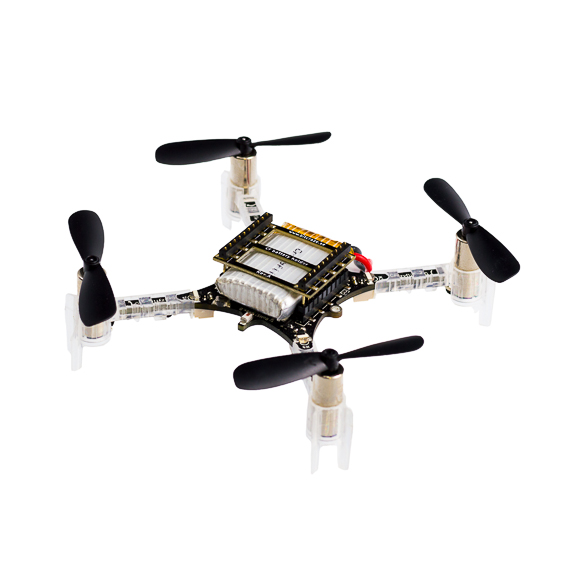
\includegraphics[scale=0.4]{figs/topic/crazyflie.jpg}};
\node[draw, above left] (time) at (phys.south east)  {\faClock[regular]};

%%% ARROWS %%%

\draw[-latex] ([yshift=0.65cm]hw.south) to node[yshift=0.85cm,rotate=90]{actuation} ([yshift=0.65cm]phys.west);
\draw[-latex] ([yshift=-0.65cm]phys.west) to node[yshift=-0.85cm, rotate=90]{sensing} ([yshift=-0.65cm]hw.south);

\end{tikzpicture}
}%
        \only<7>{\def \delta {0.15}
\def \circlesizecm {0.5cm}
\def \circleshiftcm {0.125cm}
\def \armlength {0.625}
\def \armwidthcm {0.1cm}
\def \bodywidthcm {0.5cm}

\begin{tikzpicture}
\tikzstyle{task} = [draw,thick,fill=white,align=center]
\tikzstyle{turbine} = [circle,ultra thick,draw,fill=white,minimum size=\circlesizecm,inner sep=0pt,outer sep=0pt]

%%% TASKS %%%

\node[task,opacity=0.3] (t1) at (-1.5+0*\delta,1.6-0*\delta) {\textcolor{white}{Task $\#3$} \\\textcolor{white}{\faFileCode[regular]}};
\node[task,opacity=0.6] (t2) at (-1.5+1*\delta,1.6-1*\delta) {\textcolor{white}{Task $\#2$} \\\textcolor{white}{\faFileCode[regular]}};
\node[task,opacity=1.0] (t3) at (-1.5+2*\delta,1.6-2*\delta) {Task $\#1$ \\\faFileCode[regular]};

{\color{lqgcolour}\node[task,opacity=0.3] (ct1) at (1.5+0*\delta,1.6-0*\delta) {\textcolor{white}{Control Task $\#3$} \\\textcolor{white}{\faFileCode[regular]}};}
{\color{lqgcolour}\node[task,opacity=0.6] (ct2) at (1.5+1*\delta,1.6-1*\delta) {\textcolor{white}{Control Task $\#2$} \\\textcolor{white}{\faFileCode[regular]}};}
{\color{lqgcolour}\node[task,opacity=1.0] (ct3) at (1.5+2*\delta,1.6-2*\delta) {Control Task $\#1$ \\\faFileCode[regular]};}

%%% CYBER %%%

\node[thick, align=center] (rtos) at (-0.1,0.25) {Real-Time Operating System};
\node[thick, draw, align=center, rotate=90, text width=2.75cm] (hwi) at (4.1,0.87) {HW Interfaces};
\node[thick, fit=(rtos)(t1)(ct1)(ct3),draw,yshift=1.5mm,xshift=0.75mm] (sw) {};
\node[thick, draw, above left] (clock) at (sw.south east) {\faClock[regular]};
\node[thick, fit=(sw)(hwi), inner sep=7pt, draw] (hw) {};
\node[thick, above left, xshift=2.40cm, yshift=0.5mm] (hw-label) at (hw.south west) {Hardware};
\node[thick, draw, above right] (hwclock) at (hw.south west)  {\faClock[regular]};

%%% PHYSICAL %%%

\node[task, minimum width=2.125cm, minimum height=2.125cm] (phys) at (7.0,0.875) {};
% body
\node[
    draw,
    rounded corners=3pt,
    fill=black,
    minimum width=\bodywidthcm,
    minimum height=\bodywidthcm,
    name path=B] (body) at (phys) {};

% upper left turbine
\node[turbine, anchor=south east] (dronenw) at ([xshift=-\circleshiftcm, yshift=\circleshiftcm]body.north west) {};
\draw[name path=NW] ([yshift=-\armwidthcm]body.north west)..controls($(phys) + (-\armlength, \armlength)$)..([xshift=\armwidthcm]body.north west);
\tikzfillbetween [of=NW and B] {};
\draw[fill=black, rotate=75] (dronenw) ellipse (0.175cm and 0.025cm);
\draw[fill=black, rotate=165] (dronenw) ellipse (0.175cm and 0.025cm);
        
% upper right turbine
\node[turbine, anchor=south west] (dronene) at ([xshift=\circleshiftcm, yshift=\circleshiftcm]body.north east) {};
\draw[name path=NE] ([xshift=-\armwidthcm]body.north east)..controls($(phys) + (\armlength, \armlength)$)..([yshift=-\armwidthcm]body.north east);
\tikzfillbetween [of=NE and B] {};
\draw[fill=black, rotate=75] (dronene) ellipse (0.175cm and 0.025cm);
\draw[fill=black, rotate=165] (dronene) ellipse (0.175cm and 0.025cm);

% lower right turbine
\node[turbine, anchor=north west] (dronese) at ([xshift=\circleshiftcm, yshift=-\circleshiftcm]body.south east) {};
\draw[name path=SE] ([yshift=\armwidthcm]body.south east)..controls($(phys) + (\armlength, -\armlength)$)..([xshift=-\armwidthcm]body.south east);
\tikzfillbetween [of=SE and B] {};
\draw[fill=black, rotate=75] (dronese) ellipse (0.175cm and 0.025cm);
\draw[fill=black, rotate=165] (dronese) ellipse (0.175cm and 0.025cm);

% lower left turbine
\node[turbine, anchor=north east] (dronesw) at ([xshift=-\circleshiftcm, yshift=-\circleshiftcm]body.south west) {};
\draw[name path=SW] ([xshift=\armwidthcm]body.south west)..controls($(phys) + (-\armlength, -\armlength)$)..([yshift=\armwidthcm]body.south west);
\tikzfillbetween [of=SW and B] {};
\draw[fill=black, rotate=75] (dronesw) ellipse (0.175cm and 0.025cm);
\draw[fill=black, rotate=165] (dronesw) ellipse (0.175cm and 0.025cm);

% Clock
\node[task, above left] (time) at (phys.south east) {\faClock[regular]};

%%% ARROWS %%%

\draw[thick, -latex] ([yshift=0.65cm]hwi.south) to node[yshift=0.85cm,xshift=1mm,rotate=90] {Actuation} ([yshift=0.65cm]phys.west);
\draw[thick, -latex] ([yshift=-0.65cm]phys.west) to node[yshift=-0.75cm,xshift=1mm,rotate=90] {Sensing} ([yshift=-0.65cm]hwi.south);

\end{tikzpicture}
}%
    \end{figure}
\end{frame}

\begin{frame}
    \frametitle{Markov Chain}%
    \framesubtitle{Kill}%
    \vspace{-2em}
    \begin{figure}
        \centering
        \only<1>{\def \dist {2.75}

\begin{tikzpicture}

\tikzset{Markov Node/.style={%
draw,
thick,
circle,
inner sep=0pt,
minimum size=1.5cm
}}

\node[Markov Node] (THT) at (0, 0) {\textcolor{hicolour}{\faBox}\,\textcolor{hicolour}{\faFileCode[regular]}\,\textcolor{hicolour}{\faBox}};
\node[Markov Node] (FHT) at (\dist, 0) {\textcolor{red}{\faBox}\,\textcolor{hicolour}{\faFileCode[regular]}\,\textcolor{hicolour}{\faBox}};
\node[Markov Node] (THF) at (2*\dist, 0) {\textcolor{hicolour}{\faBox}\,\textcolor{hicolour}{\faFileCode[regular]}\,\textcolor{red}{\faBox}};
\node[Markov Node] (FHF) at (3*\dist, 0) {\textcolor{red}{\faBox}\,\textcolor{hicolour}{\faFileCode[regular]}\,\textcolor{red}{\faBox}};
\node[Markov Node] (TMX) at (\dist, -1.5*\dist) {\textcolor{hicolour}{\faBox}\,\textcolor{red}{\faFileCode[regular]}\,\textcolor{black}{\faBox}};
\node[Markov Node] (FMX) at (2*\dist, -1.5*\dist) {\textcolor{red}{\faBox}\,\textcolor{red}{\faFileCode[regular]}\,\textcolor{black}{\faBox}};

\invisible{%
\node[Markov Node] at (0, 0) {\textcolor{hicolour}{\faBox}\,\textcolor{hicolour}{\faFileCode[regular]}\,\textcolor{hicolour}{\faBox}};
\node[Markov Node] at (\dist, 0) {\textcolor{red}{\faBox}\,\textcolor{hicolour}{\faFileCode[regular]}\,\textcolor{hicolour}{\faBox}};
\node[Markov Node] at (2*\dist, 0) {\textcolor{hicolour}{\faBox}\,\textcolor{hicolour}{\faFileCode[regular]}\,\textcolor{red}{\faBox}};
\node[Markov Node] at (3*\dist, 0) {\textcolor{red}{\faBox}\,\textcolor{hicolour}{\faFileCode[regular]}\,\textcolor{red}{\faBox}};
\node[Markov Node] at (\dist, -1.5*\dist) {\textcolor{hicolour}{\faBox}\,\textcolor{red}{\faFileCode[regular]}\,\textcolor{black}{\faBox}};
\node[Markov Node] at (2*\dist, -1.5*\dist) {\textcolor{red}{\faBox}\,\textcolor{red}{\faFileCode[regular]}\,\textcolor{black}{\faBox}};
}%

% straight arrows
\draw[latex-latex, thick] (THT) -- (FHT);
\draw[latex-latex, thick] (FHT) -- (THF);
\draw[latex-latex, thick] (THF) -- (FHF);
\draw[latex-latex, thick] (FHT) -- (TMX);
\draw[latex-latex, thick] (THF) -- (FMX);
\draw[latex-latex, thick] (FMX) -- (TMX);

% Bent arrows starting in THT
\draw[latex-latex, thick] (THT) to [bend left=30] (THF);
\draw[latex-latex, thick] (THT) to [bend left=37.5] (FHF);
\invisible{\draw[latex-latex, ultra thick] (THT) to [bend left=37.5] (FHF);}
\draw[latex-latex, thick] (THT) to [bend right=15] (TMX);
\draw[latex-latex, thick] (THT) to [bend right=5] (FMX);

% Bent arrows starting in FHT
\draw[latex-latex, thick] (FHT) to [bend left=30] (FHF);
\draw[latex-latex, thick] (FHT) to [bend right=10] (FMX);

% Bent arrows starting in THF
\draw[latex-latex, thick] (THF) to [bend left=10] (TMX);

% Bent arrows starting in FHF
\draw[latex-latex, thick] (FHF) to [bend left=15] (FMX);
\draw[latex-latex, thick] (FHF) to [bend left=5] (TMX);

\end{tikzpicture}
}%
        \only<2>{\def \dist {2.75}

\begin{tikzpicture}

\tikzset{Markov Node/.style={%
draw,
thick,
circle,
inner sep=0pt,
minimum size=1.5cm
}}

\node[Markov Node, ultra thick, hicolour] (THT) at (0, 0) {\textcolor{hicolour}{\faBox}\,\textcolor{hicolour}{\faFileCode[regular]}\,\textcolor{hicolour}{\faBox}};
\node[Markov Node] (FHT) at (\dist, 0) {\textcolor{red}{\faBox}\,\textcolor{hicolour}{\faFileCode[regular]}\,\textcolor{hicolour}{\faBox}};
\node[Markov Node] (THF) at (2*\dist, 0) {\textcolor{hicolour}{\faBox}\,\textcolor{hicolour}{\faFileCode[regular]}\,\textcolor{red}{\faBox}};
\node[Markov Node] (FHF) at (3*\dist, 0) {\textcolor{red}{\faBox}\,\textcolor{hicolour}{\faFileCode[regular]}\,\textcolor{red}{\faBox}};
\node[Markov Node] (TMX) at (\dist, -1.5*\dist) {\textcolor{hicolour}{\faBox}\,\textcolor{red}{\faFileCode[regular]}\,\textcolor{black}{\faBox}};
\node[Markov Node] (FMX) at (2*\dist, -1.5*\dist) {\textcolor{red}{\faBox}\,\textcolor{red}{\faFileCode[regular]}\,\textcolor{black}{\faBox}};

\invisible{%
\node[Markov Node] at (0, 0) {\textcolor{hicolour}{\faBox}\,\textcolor{hicolour}{\faFileCode[regular]}\,\textcolor{hicolour}{\faBox}};
\node[Markov Node] at (\dist, 0) {\textcolor{red}{\faBox}\,\textcolor{hicolour}{\faFileCode[regular]}\,\textcolor{hicolour}{\faBox}};
\node[Markov Node] at (2*\dist, 0) {\textcolor{hicolour}{\faBox}\,\textcolor{hicolour}{\faFileCode[regular]}\,\textcolor{red}{\faBox}};
\node[Markov Node] at (3*\dist, 0) {\textcolor{red}{\faBox}\,\textcolor{hicolour}{\faFileCode[regular]}\,\textcolor{red}{\faBox}};
\node[Markov Node] at (\dist, -1.5*\dist) {\textcolor{hicolour}{\faBox}\,\textcolor{red}{\faFileCode[regular]}\,\textcolor{black}{\faBox}};
\node[Markov Node] at (2*\dist, -1.5*\dist) {\textcolor{red}{\faBox}\,\textcolor{red}{\faFileCode[regular]}\,\textcolor{black}{\faBox}};
}%

% straight arrows
\draw[latex-latex, thick] (THT) -- (FHT);
\draw[latex-latex, thick] (FHT) -- (THF);
\draw[latex-latex, thick] (THF) -- (FHF);
\draw[latex-latex, thick] (FHT) -- (TMX);
\draw[latex-latex, thick] (THF) -- (FMX);
\draw[latex-latex, thick] (FMX) -- (TMX);

% Bent arrows starting in THT
\draw[latex-latex, thick] (THT) to [bend left=30] (THF);
\draw[latex-latex, ultra thick, hicolour] (THT) to [bend left=37.5] (FHF);
\invisible{\draw[latex-latex, ultra thick] (THT) to [bend left=37.5] (FHF);}
\draw[latex-latex, thick] (THT) to [bend right=15] (TMX);
\draw[latex-latex, thick] (THT) to [bend right=5] (FMX);

% Bent arrows starting in FHT
\draw[latex-latex, thick] (FHT) to [bend left=30] (FHF);
\draw[latex-latex, thick] (FHT) to [bend right=10] (FMX);

% Bent arrows starting in THF
\draw[latex-latex, thick] (THF) to [bend left=10] (TMX);

% Bent arrows starting in FHF
\draw[latex-latex, thick] (FHF) to [bend left=15] (FMX);
\draw[latex-latex, thick] (FHF) to [bend left=5] (TMX);

\end{tikzpicture}
}%
        \only<3>{\def \dist {2.75}

\begin{tikzpicture}

\tikzset{Markov Node/.style={%
draw,
thick,
circle,
inner sep=0pt,
minimum size=1.5cm
}}

\node[Markov Node] (THT) at (0, 0) {\textcolor{hicolour}{\faBox}\,\textcolor{hicolour}{\faFileCode[regular]}\,\textcolor{hicolour}{\faBox}};
\node[Markov Node] (FHT) at (\dist, 0) {\textcolor{red}{\faBox}\,\textcolor{hicolour}{\faFileCode[regular]}\,\textcolor{hicolour}{\faBox}};
\node[Markov Node] (THF) at (2*\dist, 0) {\textcolor{hicolour}{\faBox}\,\textcolor{hicolour}{\faFileCode[regular]}\,\textcolor{red}{\faBox}};
\node[Markov Node, ultra thick, hicolour] (FHF) at (3*\dist, 0) {\textcolor{red}{\faBox}\,\textcolor{hicolour}{\faFileCode[regular]}\,\textcolor{red}{\faBox}};
\node[Markov Node] (TMX) at (\dist, -1.5*\dist) {\textcolor{hicolour}{\faBox}\,\textcolor{red}{\faFileCode[regular]}\,\textcolor{black}{\faBox}};
\node[Markov Node] (FMX) at (2*\dist, -1.5*\dist) {\textcolor{red}{\faBox}\,\textcolor{red}{\faFileCode[regular]}\,\textcolor{black}{\faBox}};

% straight arrows
\draw[latex-latex, thick] (THT) -- (FHT);
\draw[latex-latex, thick] (FHT) -- (THF);
\draw[latex-latex, thick] (THF) -- (FHF);
\draw[latex-latex, thick] (FHT) -- (TMX);
\draw[latex-latex, thick] (THF) -- (FMX);
\draw[latex-latex, thick] (FMX) -- (TMX);

% Bent arrows starting in THT
\draw[latex-latex, thick] (THT) to [bend left=30] (THF);
\draw[latex-latex, thick] (THT) to [bend left=37.5] (FHF);
\draw[latex-latex, thick] (THT) to [bend right=15] (TMX);
\draw[latex-latex, thick] (THT) to [bend right=5] (FMX);

% Bent arrows starting in FHT
\draw[latex-latex, thick] (FHT) to [bend left=30] (FHF);
\draw[latex-latex, thick] (FHT) to [bend right=10] (FMX);

% Bent arrows starting in THF
\draw[latex-latex, thick] (THF) to [bend left=10] (TMX);

% Bent arrows starting in FHF
\draw[latex-latex, ultra thick, hicolour] (FHF) to [bend left=15] (FMX);
\draw[latex-latex, thick] (FHF) to [bend left=5] (TMX);

\end{tikzpicture}
}%
        \only<4>{\def \dist {2.75}

\begin{tikzpicture}

\tikzset{Markov Node/.style={%
draw,
thick,
circle,
inner sep=0pt,
minimum size=1.5cm
}}

\node[Markov Node] (THT) at (0, 0) {\textcolor{hicolour}{\faBox}\,\textcolor{hicolour}{\faFileCode[regular]}\,\textcolor{hicolour}{\faBox}};
\node[Markov Node] (FHT) at (\dist, 0) {\textcolor{red}{\faBox}\,\textcolor{hicolour}{\faFileCode[regular]}\,\textcolor{hicolour}{\faBox}};
\node[Markov Node] (THF) at (2*\dist, 0) {\textcolor{hicolour}{\faBox}\,\textcolor{hicolour}{\faFileCode[regular]}\,\textcolor{red}{\faBox}};
\node[Markov Node] (FHF) at (3*\dist, 0) {\textcolor{red}{\faBox}\,\textcolor{hicolour}{\faFileCode[regular]}\,\textcolor{red}{\faBox}};
\node[Markov Node] (TMX) at (\dist, -1.5*\dist) {\textcolor{hicolour}{\faBox}\,\textcolor{red}{\faFileCode[regular]}\,\textcolor{black}{\faBox}};
\node[Markov Node, ultra thick, hicolour] (FMX) at (2*\dist, -1.5*\dist) {\textcolor{red}{\faBox}\,\textcolor{red}{\faFileCode[regular]}\,\textcolor{black}{\faBox}};

\invisible{%
\node[Markov Node] at (0, 0) {\textcolor{hicolour}{\faBox}\,\textcolor{hicolour}{\faFileCode[regular]}\,\textcolor{hicolour}{\faBox}};
\node[Markov Node] at (\dist, 0) {\textcolor{red}{\faBox}\,\textcolor{hicolour}{\faFileCode[regular]}\,\textcolor{hicolour}{\faBox}};
\node[Markov Node] at (2*\dist, 0) {\textcolor{hicolour}{\faBox}\,\textcolor{hicolour}{\faFileCode[regular]}\,\textcolor{red}{\faBox}};
\node[Markov Node] at (3*\dist, 0) {\textcolor{red}{\faBox}\,\textcolor{hicolour}{\faFileCode[regular]}\,\textcolor{red}{\faBox}};
\node[Markov Node] at (\dist, -1.5*\dist) {\textcolor{hicolour}{\faBox}\,\textcolor{red}{\faFileCode[regular]}\,\textcolor{black}{\faBox}};
\node[Markov Node] at (2*\dist, -1.5*\dist) {\textcolor{red}{\faBox}\,\textcolor{red}{\faFileCode[regular]}\,\textcolor{black}{\faBox}};
}%

% straight arrows
\draw[latex-latex, thick] (THT) -- (FHT);
\draw[latex-latex, thick] (FHT) -- (THF);
\draw[latex-latex, thick] (THF) -- (FHF);
\draw[latex-latex, thick] (FHT) -- (TMX);
\draw[latex-latex, thick] (THF) -- (FMX);
\draw[latex-latex, ultra thick, hicolour] (FMX) -- (TMX);

% Bent arrows starting in THT
\draw[latex-latex, thick] (THT) to [bend left=30] (THF);
\draw[latex-latex, thick] (THT) to [bend left=37.5] (FHF);
\invisible{\draw[latex-latex, ultra thick] (THT) to [bend left=37.5] (FHF);}
\draw[latex-latex, thick] (THT) to [bend right=15] (TMX);
\draw[latex-latex, thick] (THT) to [bend right=5] (FMX);

% Bent arrows starting in FHT
\draw[latex-latex, thick] (FHT) to [bend left=30] (FHF);
\draw[latex-latex, thick] (FHT) to [bend right=10] (FMX);

% Bent arrows starting in THF
\draw[latex-latex, thick] (THF) to [bend left=10] (TMX);

% Bent arrows starting in FHF
\draw[latex-latex, thick] (FHF) to [bend left=15] (FMX);
\draw[latex-latex, thick] (FHF) to [bend left=5] (TMX);

\end{tikzpicture}
}%
        \only<5>{\def \dist {2.75}

\begin{tikzpicture}

\tikzset{Markov Node/.style={%
draw,
thick,
circle,
inner sep=0pt,
minimum size=1.5cm
}}

\node[Markov Node] (THT) at (0, 0) {\textcolor{hicolour}{\faBox}\,\textcolor{hicolour}{\faFileCode[regular]}\,\textcolor{hicolour}{\faBox}};
\node[Markov Node] (FHT) at (\dist, 0) {\textcolor{red}{\faBox}\,\textcolor{hicolour}{\faFileCode[regular]}\,\textcolor{hicolour}{\faBox}};
\node[Markov Node] (THF) at (2*\dist, 0) {\textcolor{hicolour}{\faBox}\,\textcolor{hicolour}{\faFileCode[regular]}\,\textcolor{red}{\faBox}};
\node[Markov Node] (FHF) at (3*\dist, 0) {\textcolor{red}{\faBox}\,\textcolor{hicolour}{\faFileCode[regular]}\,\textcolor{red}{\faBox}};
\node[Markov Node, ultra thick, hicolour] (TMX) at (\dist, -1.5*\dist) {\textcolor{hicolour}{\faBox}\,\textcolor{red}{\faFileCode[regular]}\,\textcolor{black}{\faBox}};
\node[Markov Node] (FMX) at (2*\dist, -1.5*\dist) {\textcolor{red}{\faBox}\,\textcolor{red}{\faFileCode[regular]}\,\textcolor{black}{\faBox}};

\invisible{%
\node[Markov Node] at (0, 0) {\textcolor{hicolour}{\faBox}\,\textcolor{hicolour}{\faFileCode[regular]}\,\textcolor{hicolour}{\faBox}};
\node[Markov Node] at (\dist, 0) {\textcolor{red}{\faBox}\,\textcolor{hicolour}{\faFileCode[regular]}\,\textcolor{hicolour}{\faBox}};
\node[Markov Node] at (2*\dist, 0) {\textcolor{hicolour}{\faBox}\,\textcolor{hicolour}{\faFileCode[regular]}\,\textcolor{red}{\faBox}};
\node[Markov Node] at (3*\dist, 0) {\textcolor{red}{\faBox}\,\textcolor{hicolour}{\faFileCode[regular]}\,\textcolor{red}{\faBox}};
\node[Markov Node] at (\dist, -1.5*\dist) {\textcolor{hicolour}{\faBox}\,\textcolor{red}{\faFileCode[regular]}\,\textcolor{black}{\faBox}};
\node[Markov Node] at (2*\dist, -1.5*\dist) {\textcolor{red}{\faBox}\,\textcolor{red}{\faFileCode[regular]}\,\textcolor{black}{\faBox}};
}%

% straight arrows
\draw[latex-latex, thick] (THT) -- (FHT);
\draw[latex-latex, thick] (FHT) -- (THF);
\draw[latex-latex, thick] (THF) -- (FHF);
\draw[latex-latex, ultra thick, hicolour] (FHT) -- (TMX);
\draw[latex-latex, thick] (THF) -- (FMX);
\draw[latex-latex, thick] (FMX) -- (TMX);

% Bent arrows starting in THT
\draw[latex-latex, thick] (THT) to [bend left=30] (THF);
\draw[latex-latex, thick] (THT) to [bend left=37.5] (FHF);
\invisible{\draw[latex-latex, ultra thick] (THT) to [bend left=37.5] (FHF);}
\draw[latex-latex, thick] (THT) to [bend right=15] (TMX);
\draw[latex-latex, thick] (THT) to [bend right=5] (FMX);

% Bent arrows starting in FHT
\draw[latex-latex, thick] (FHT) to [bend left=30] (FHF);
\draw[latex-latex, thick] (FHT) to [bend right=10] (FMX);

% Bent arrows starting in THF
\draw[latex-latex, thick] (THF) to [bend left=10] (TMX);

% Bent arrows starting in FHF
\draw[latex-latex, thick] (FHF) to [bend left=15] (FMX);
\draw[latex-latex, thick] (FHF) to [bend left=5] (TMX);

\end{tikzpicture}
}%
    \end{figure}
\end{frame}
